\documentclass{amsart}\usepackage[]{graphicx}\usepackage[]{color}
%% maxwidth is the original width if it is less than linewidth
%% otherwise use linewidth (to make sure the graphics do not exceed the margin)
\makeatletter
\def\maxwidth{ %
  \ifdim\Gin@nat@width>\linewidth
    \linewidth
  \else
    \Gin@nat@width
  \fi
}
\makeatother

\definecolor{fgcolor}{rgb}{0.345, 0.345, 0.345}
\newcommand{\hlnum}[1]{\textcolor[rgb]{0.686,0.059,0.569}{#1}}%
\newcommand{\hlstr}[1]{\textcolor[rgb]{0.192,0.494,0.8}{#1}}%
\newcommand{\hlcom}[1]{\textcolor[rgb]{0.678,0.584,0.686}{\textit{#1}}}%
\newcommand{\hlopt}[1]{\textcolor[rgb]{0,0,0}{#1}}%
\newcommand{\hlstd}[1]{\textcolor[rgb]{0.345,0.345,0.345}{#1}}%
\newcommand{\hlkwa}[1]{\textcolor[rgb]{0.161,0.373,0.58}{\textbf{#1}}}%
\newcommand{\hlkwb}[1]{\textcolor[rgb]{0.69,0.353,0.396}{#1}}%
\newcommand{\hlkwc}[1]{\textcolor[rgb]{0.333,0.667,0.333}{#1}}%
\newcommand{\hlkwd}[1]{\textcolor[rgb]{0.737,0.353,0.396}{\textbf{#1}}}%
\let\hlipl\hlkwb

\usepackage{framed}
\makeatletter
\newenvironment{kframe}{%
 \def\at@end@of@kframe{}%
 \ifinner\ifhmode%
  \def\at@end@of@kframe{\end{minipage}}%
  \begin{minipage}{\columnwidth}%
 \fi\fi%
 \def\FrameCommand##1{\hskip\@totalleftmargin \hskip-\fboxsep
 \colorbox{shadecolor}{##1}\hskip-\fboxsep
     % There is no \\@totalrightmargin, so:
     \hskip-\linewidth \hskip-\@totalleftmargin \hskip\columnwidth}%
 \MakeFramed {\advance\hsize-\width
   \@totalleftmargin\z@ \linewidth\hsize
   \@setminipage}}%
 {\par\unskip\endMakeFramed%
 \at@end@of@kframe}
\makeatother

\definecolor{shadecolor}{rgb}{.97, .97, .97}
\definecolor{messagecolor}{rgb}{0, 0, 0}
\definecolor{warningcolor}{rgb}{1, 0, 1}
\definecolor{errorcolor}{rgb}{1, 0, 0}
\newenvironment{knitrout}{}{} % an empty environment to be redefined in TeX

\usepackage{alltt}
	%% Basic Info
		\author{Alex Thies}
		\title{Final Exam \\ Math 463 - Spring 2017}
		\email{athies@uoregon.edu}
	%% boilerplate packages
		\usepackage{amsmath}
		\usepackage{amssymb}
		\usepackage{amsthm}
		\usepackage{enumerate}
		\usepackage{mathrsfs}
		\usepackage{color}
		\usepackage{hyperref}
	%% rename the abstract
		\renewcommand{\abstractname}{Introduction}
	%% my shorthand
		% sets
		\DeclareMathOperator{\Z}{\mathbb{Z}}
		\DeclareMathOperator{\Zp}{\mathbb{Z^{+}}}
		\DeclareMathOperator{\Zm}{\mathbb{Z^{-}}}
		\DeclareMathOperator{\N}{\mathbb{Z^{+}}}
		% linear algebra stuff
		\DeclareMathOperator{\Ell}{\mathscr{L}}
		% stats stuff
		\DeclareMathOperator{\var}{\rm Var}
		\DeclareMathOperator{\cov}{\rm Cov}
		\DeclareMathOperator{\sd}{\rm SD}
		\DeclareMathOperator{\SE}{\rm SE}
		\DeclareMathOperator{\ind}{\perp\!\!\!\perp}
		\DeclareMathOperator{\Prob}{\mathbb{P}}
		% use pretty characters
		\DeclareMathOperator{\ep}{\varepsilon}
		\DeclareMathOperator{\ph}{\varphi}
	%% Levin's shorthand
		\newcommand{\E}{{\mathcal{E}}}
		\newcommand{\A}{{\mathcal{A}}}
		\newcommand{\B}{{\mathcal{B}}}
		\newcommand{\R}{{\mathbb{R}}}
		\newcommand{\X}{{\mathbf{X}}}
		\newcommand{\x}{{\mathbf{x}}}
		\newcommand{\M}{{\mathcal{M}}}
		\newcommand{\bvec}[1]{{\boldsymbol #1}}
		\newcommand{\bbeta}{\bvec{\beta}}
		\newcommand{\bX}{\bvec{X}}
		\newcommand{\bY}{\bvec{Y}}
		\newcommand{\ssreg}{{\rm SS}_{{\rm Reg}}}
		\newcommand{\ssr}{{\rm SS}_{{\rm Res}}}
		\newcommand{\sst}{{\rm SS}_{{\rm Tot}}}
\IfFileExists{upquote.sty}{\usepackage{upquote}}{}
\begin{document}
	\begin{abstract}
		By submitting this final, I certify that I have followed exactly the rules outlined on the front of the exam.
	\end{abstract}

	\maketitle

	\section{Assignment} % (fold)
	\label{sec:assignment}
		\subsection{Problem 1} % (fold)
		\label{sub:problem_1}
		Consider the data available at
\begin{knitrout}
\definecolor{shadecolor}{rgb}{0.969, 0.969, 0.969}\color{fgcolor}\begin{kframe}
\begin{alltt}
\hlkwd{rm}\hlstd{(}\hlkwc{list}\hlstd{=}\hlkwd{ls}\hlstd{())}
\hlstd{ozone} \hlkwb{<-} \hlkwd{read.table}\hlstd{(}\hlstr{"http://pages.uoregon.edu/dlevin/DATA/ozo.txt"}\hlstd{,}
                    \hlkwc{header}\hlstd{=T)}
\end{alltt}
\end{kframe}
\end{knitrout}
		The variables \verb|temp| and \verb|humidity| give daily temperature and humidity readings.
		The variable \verb|HO| indicates if ozone levels are high.
		Use the data to fit a probit model:
		Here let $Y_i = 1$ if and only if the ozone level is high, and write $\bvec{x}^{(i)} = (1, {\tt temp}_i, {\tt humidity}_i)$.
		\[
		\Prob(Y_i = 1 \mid \bvec{x}^{(i)}) = \Phi( \bvec{x}^{(i)} \bvec{\beta}) \,,
		\]
		where $\Phi$ is the normal cdf.
		Provide the fitted coefficients and their standard errors.
		(The R function \verb|glm| can be used to fit a probit. Be sure to specify \verb|family=binomial(link="probit")|.)
		\begin{enumerate}[(a)]
		\item What is the estimated probability of a high ozone day if the temperature is 95 degrees and the humidity is 80\%?
		\item Find a 95\% confidence interval for the linear predictor $\beta_0 + 95\beta_1 + 80\beta_2$ at these values.
		\item Find a 95\% confidence interval for the probability  of high ozone at these values.
		\end{enumerate}
		Note that if \verb|f| is the fitted probit model (using \verb|glm|), then \verb|summary(f)$cov.unscaled| gives the approximate covariance matrix $\cov(\hat{\bvec{\beta}})$.
		Alternatively, \verb|predict| can give fitted values and their standard errors, for given covariates.
		\begin{proof}[Solution] \

			\begin{enumerate}[(a)]
				\item We compute the following in R,
				    \begin{align*}
				        \Prob(X\beta | \beta_{\rm Temp} = 95, \beta_{\rm Humid} = 80) &= \Phi(x_{0} + \beta_{\rm Temp}x_{1} + \beta_{\rm Humid}x_{2}), \\
				        &= 0.98.
				    \end{align*}
				\item We compute a 95\% following confidence interval for $X\beta$ given the specified values for temperature and humidity in R, $$\left( 1.52, 2.74 \right).$$
				\item Utilizing the endpoints of the previous confidence interval, we compute the following 95\% confidence interval for high ozone given the values of temperature and humidity, $$ \left( \Phi(1.52), \Phi(2.74) \right) = \left( 0.94, 1 \right).$$
			\end{enumerate}
		\end{proof}
		% subsubsection problem_1 (end)
		\newpage

		\subsection{Problem 2} % (fold)
		\label{sub:problem_2}

        \begin{figure}[h]
\begin{knitrout}
\definecolor{shadecolor}{rgb}{0.969, 0.969, 0.969}\color{fgcolor}
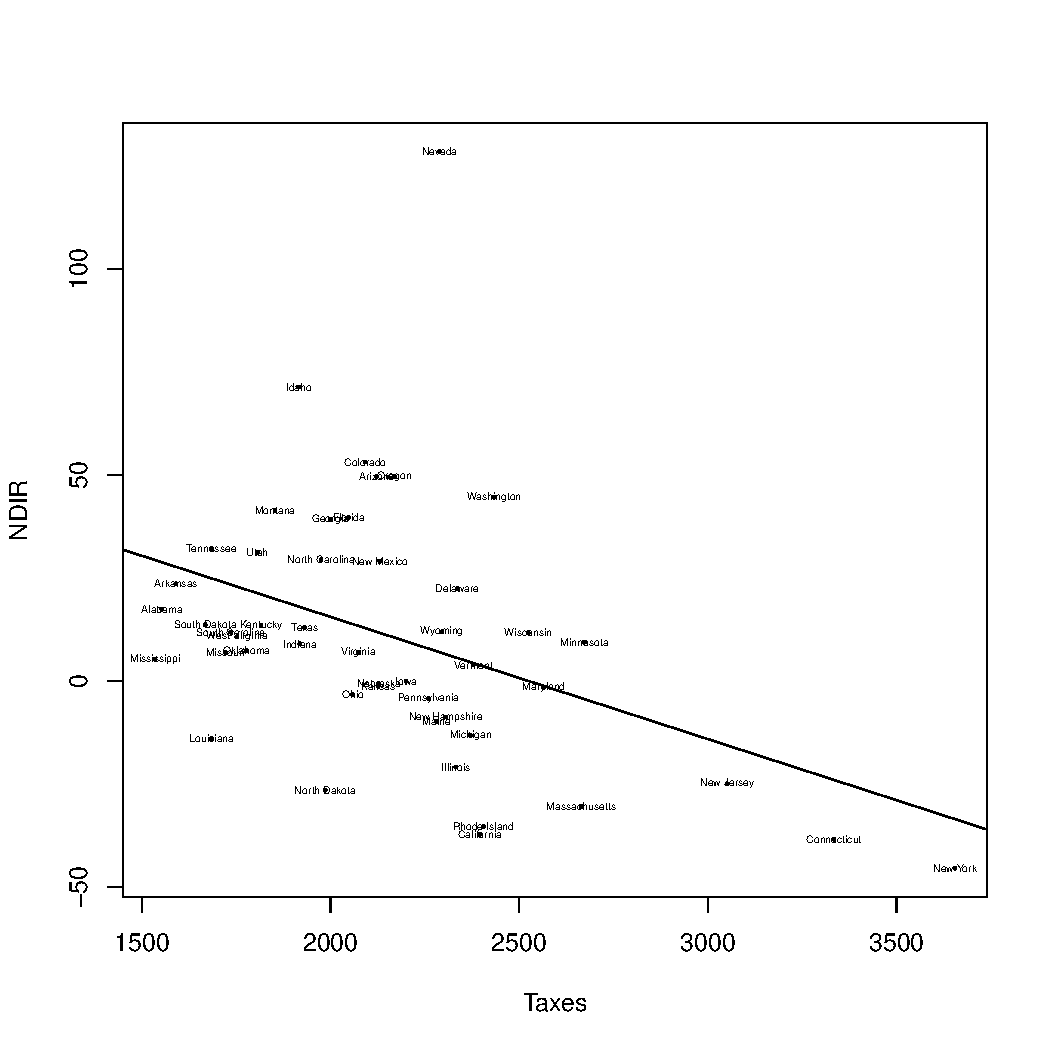
\includegraphics[width=.7\linewidth]{figure/2_Fig1-1} 

\end{knitrout}
        \caption{Immigration vs. taxes}
        \end{figure}
		This problem concerns the data available at the location specified in the R code below:

        \verb|> di = read.table("http://pages.uoregon.edu/dlevin/DATA/DI.txt",|

        \verb|+                 header=T,row.names=1,sep="\t")|

        \verb|> plot(NDIR~Taxes, data=di, pch=19, cex=0.2)|

        \verb|> text(di$Taxes,di$NDIR,row.names(di), cex=0.4)|

        \verb|> g = lm(NDIR~Taxes, data=di)|

        \verb|> abline(g)|

		Figure 1 is a scatterplot of net immigration to states against income tax.
		(The data is aggregrated over a few years in the early 90's.)
		Do people move because of tax rates?
		Use the data in the file (see above) to discuss this question.
		\begin{proof}[Solution]
		Upon inspection of the regression of Taxes onto NDIR illustrated in 1, we observe that there appears to be negative correlation.
		Looking at the summary of this model (Table 1) we observe that none of the variables are highly significant, including taxes.
% latex table generated in R 3.4.0 by xtable 1.8-2 package
% Wed Jun 14 15:21:50 2017
\begin{table}[ht]
\centering
\begin{tabular}{rrrrr}
  \hline
 & Estimate & Std. Error & t value & Pr($>$$|$t$|$) \\ 
  \hline
(Intercept) & 82.1620 & 152.5896 & 0.54 & 0.5938 \\ 
  Unemp & -1.4120 & 5.3201 & -0.27 & 0.7923 \\ 
  Wage & -0.3928 & 4.1049 & -0.10 & 0.9243 \\ 
  Crime & 0.0196 & 0.0249 & 0.79 & 0.4373 \\ 
  Income & -0.0018 & 0.0020 & -0.88 & 0.3832 \\ 
  Metrop & -0.0058 & 0.3610 & -0.02 & 0.9872 \\ 
  Poor & -2.5828 & 2.2324 & -1.16 & 0.2554 \\ 
  Taxes & -0.0131 & 0.0180 & -0.73 & 0.4723 \\ 
  Educ & 0.6199 & 1.7484 & 0.35 & 0.7251 \\ 
  BusFail & 14.9455 & 48.3529 & 0.31 & 0.7591 \\ 
  Temp & -0.2168 & 1.2619 & -0.17 & 0.8646 \\ 
  RegionNortheast & -16.8286 & 17.7235 & -0.95 & 0.3491 \\ 
  RegionSouth & 16.5672 & 16.7952 & 0.99 & 0.3309 \\ 
  RegionWest & 36.8358 & 13.8137 & 2.67 & 0.0116 \\ 
   \hline
\end{tabular}
\caption{Summary of Big Model} 
\label{Summary of Big Model}
\end{table}

		Imagine you are an overly taxed New Yorker looking to move, are you more likely to traverse the Continental United States for a lessened tax burden, or over the border say Pennsylvania, or Vermont?
		Suppose we treat region as a categorical variable and fit different slopes and intercepts according to region.
		\begin{figure}[h]
\begin{knitrout}
\definecolor{shadecolor}{rgb}{0.969, 0.969, 0.969}\color{fgcolor}
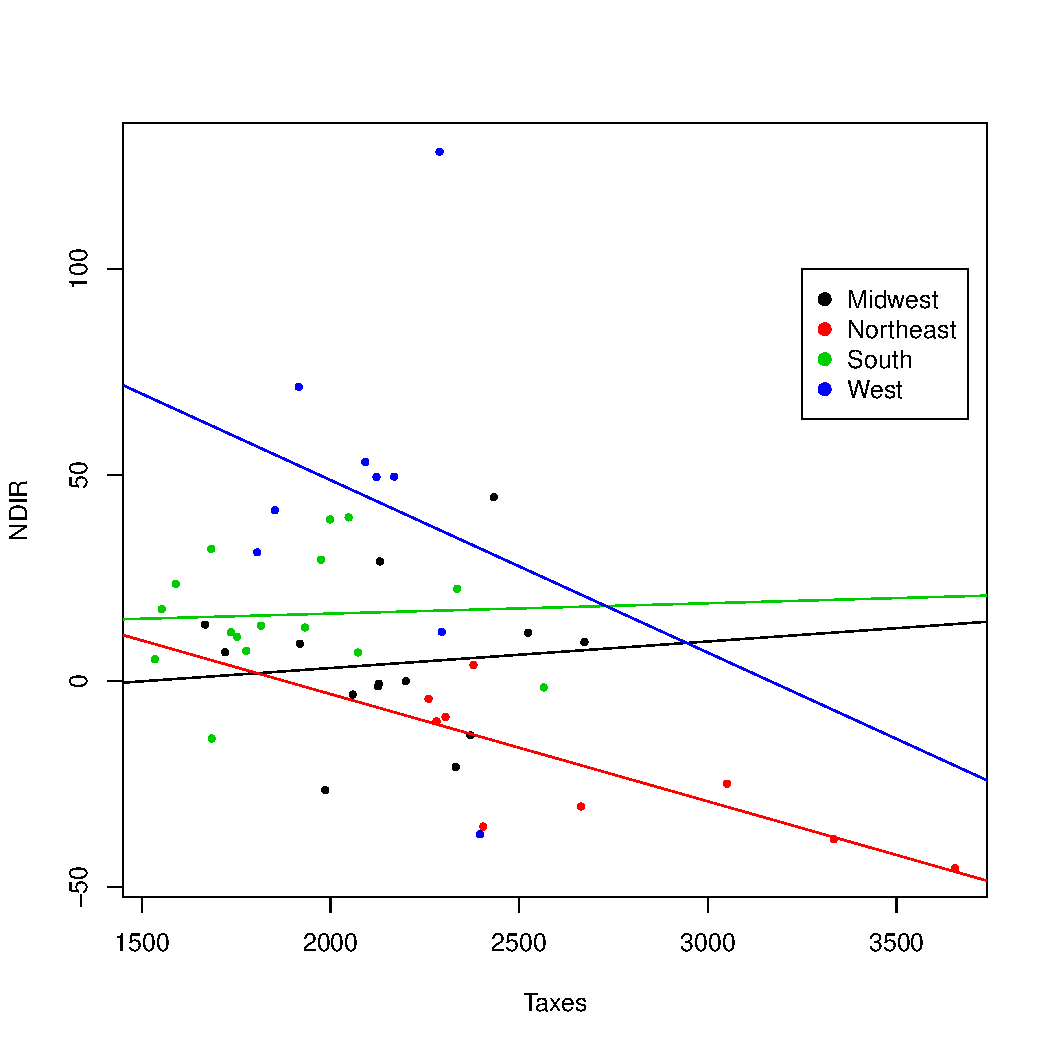
\includegraphics[width=.7\linewidth]{figure/2_Fig2-1} 

\end{knitrout}
        \caption{Immigration vs. taxes, by region}
        \end{figure}
        Figure 2 seems to indicate that one's tax burden will spur them to move, depending on where they live.
        Figure 3 illustrates that the regions which are experiencing the most out-migration are the two regions which have the highest tax burden in favor of regions with a lower tax burden.
        We can observe the ANOVA table in Table 2 to see that indeed, when split by the category of region, people may in fact move because of taxes.
% latex table generated in R 3.4.0 by xtable 1.8-2 package
% Wed Jun 14 15:21:51 2017
\begin{table}[ht]
\centering
\begin{tabular}{lrrrrrr}
  \hline
 & Res.Df & RSS & Df & Sum of Sq & F & Pr($>$F) \\ 
  \hline
1 & 47 & 46469.15 &  &  &  &  \\ 
  2 & 46 & 38769.06 & 1 & 7700.09 & 12.98 & 0.0009 \\ 
  3 & 43 & 25089.12 & 3 & 13679.94 & 7.69 & 0.0004 \\ 
  4 & 40 & 23733.04 & 3 & 1356.08 & 0.76 & 0.5222 \\ 
   \hline
\end{tabular}
\caption{ANOVA} 
\label{ANOVA}
\end{table}

        \begin{figure}[h]
\begin{knitrout}
\definecolor{shadecolor}{rgb}{0.969, 0.969, 0.969}\color{fgcolor}
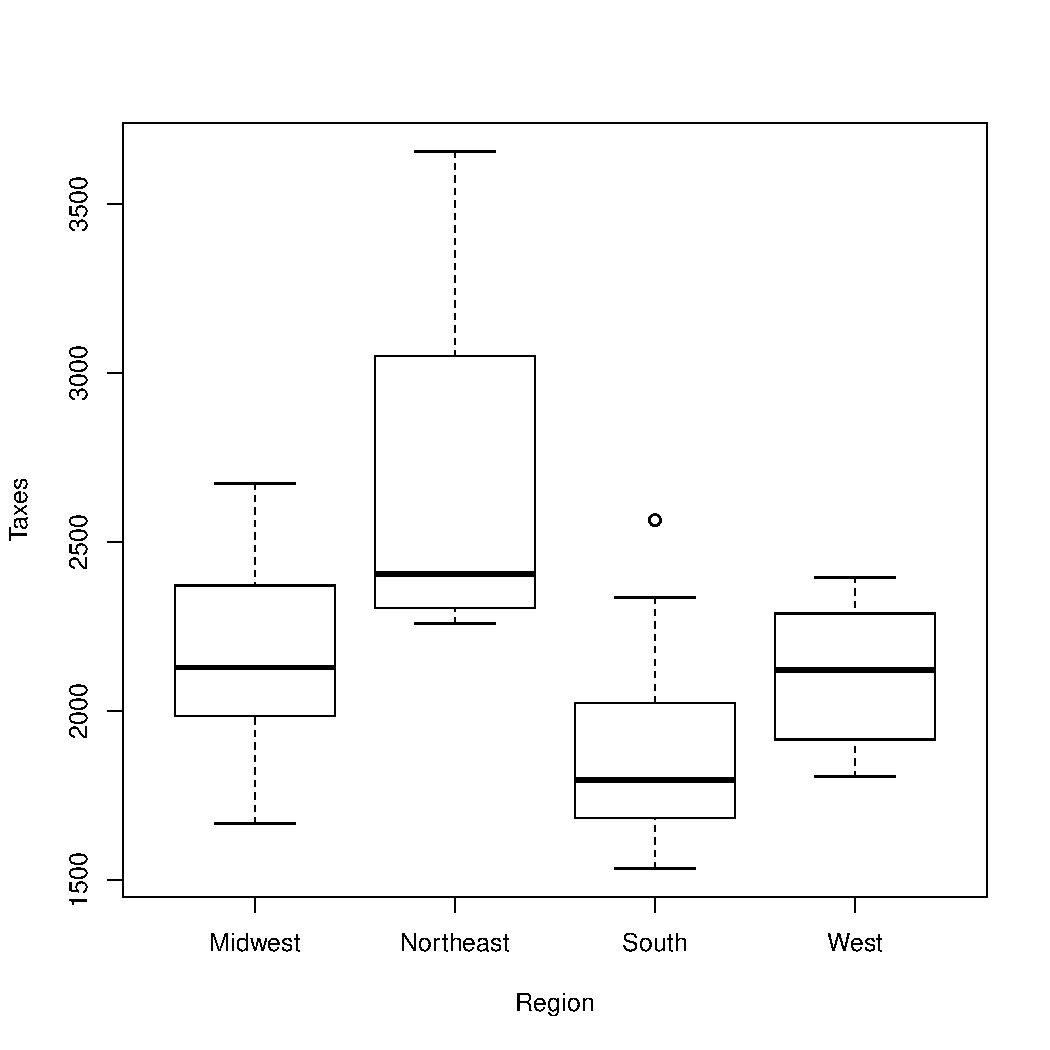
\includegraphics[width=.7\linewidth]{figure/2_Fig3-1} 

\end{knitrout}
        \caption{Region as Taxes}
        \end{figure}
        Some concerns that I have with the data in question are that factors such as income and wage may be correlated, if not linearly then in some fashion.
        I have the same concern with unemployment, business failure rate, and education.
        It also seems likely that the errors here are not necessarily independent of the variables.
        Many things have an effect on factors such as business failure rate, and education that are not taken into consideration by the model.
        Moreover, factors which might serve to answer the question posed in this problem could be things like the rate of change of the GDP of a state, the robust-ness of the welfare state, and the type of taxes which are being summed into the taxes variable.
        It seems unlikely that renters would be effected by increases in property tax, whereas they would be effected by increases in income, or sales tax.
        This question may be more easily answered given a newer set of observational data, especially given that Kansas has recently undergone massive tax cuts, effectively running an experiment for us.
		\end{proof}
		% subsection problem_2 (end)
		\newpage

		\subsection{Problem 3} % (fold)
		\label{sub:problem_3}
		Recall that Instrumental Variables Least Squares (IVLS) requires variables $\bvec{Z}$ which are independent of the error terms $\bvec{\ep}$.
		(Such variables are called \emph{exogenous}.)
		Succesful application hinges on this assumption.
		Can this be verified from the data?
		This problem explores this question.
		Suppose that
		\begin{equation} \label{Eq:YXE}
		\bvec{Y} = \bvec{Z}\bvec{\alpha} + \bvec{X}\bvec{\beta} + \bvec{\ep} \,.
		\end{equation}
		Assume $\mathbb{E}[\bvec{\ep}] = 0$.
		Let $\bvec{Z}$ be a random $n$-vector, and suppose that $\cov(Z_i,\ep_i) = \rho$.
		The triples $(Z_i,X_i,\ep_i)$ are i.i.d. as triples for $i=1,2,\ldots,n$.
		\begin{enumerate}[(a)]
		\item Show that	\begin{equation} \label{Eq:Zep}	n^{-1} \sum_{i=1}^n Z_i \ep_i \to \rho \,. \end{equation}
		\item Show that if $n$ is large enough, \emph{and you can observe $\bvec{\ep}$}, you can test $H_0: \rho = 0$ with power $0.99$ against the alternative $H_1: |\rho| > 0.001$.
		\emph{Hint}: By the CLT, the test statistic
		\[
		\sqrt{n}\left( n^{-1} \sum_{i=1}^n Z_i \ep_i - \rho \right) \approx N(0,\kappa)
		\]
		where $\kappa = \var(Z_1\ep_1)$.
		Thus, with enough data, you can determine with high probability if the errors $\bvec{\ep}$ are correlated with $\bvec{Z}$.
		(Provided you can observe $\bvec{\ep}$.
		In most applications, $\bvec{\ep}$ is unobservable, however.)
		\item Let $\bvec{e}$ be the residuals from the OLS fit in \eqref{Eq:YXE}.
		Find the limit
		\[
		\lim_{n \to \infty} n^{-1} \sum_{i=1}^n Z_i e_i = \lim_{n \to \infty} n^{-1} \langle \bvec{Z}, \bvec{e} \rangle \,.
		\]
		Is it the same as the limit in \eqref{Eq:Zep}?
		\item Can you then use the residuals $\bvec{e}$ to determine $\cov(Z_1,\ep_1)$?
		\item If ``no'' what does this say about the ability to verify exogeniety (independence from error term) of instrumental variables?
		\end{enumerate}
		\begin{proof}[Solution] \
			\begin{enumerate}[(a)]
				\item
				\item
				\item
				\item
				\item
			\end{enumerate}
		\end{proof}
		% subsection problem_3 (end)
        \newpage

		\subsection{Problem 4} % (fold)
		\label{sub:problem_4}
		Suppose that
		\[
		\bvec{Y} = \bvec{X}\bvec{\beta} + \bvec{\ep}\,.
		\]
		The variables $\bvec{Z}_1, \bvec{Z}_2$ are instruments used to estimate $\bvec{\beta}$.
		Let $\tilde{\bvec{\beta}}$ denote the IVLS estimator of $\bvec{\beta}$.
		Let $\hat{\bvec{\beta}}$ denote the OLS estimator of $\bvec{\beta}$.
		\begin{enumerate}[(a)]
		\item If $n = 10, \bvec{\beta} = (0.2,0.5)$ and $\sigma = 1$, use simulation to estimate the mean-square error of both $\tilde{\bvec{\beta}}$ and $\hat{\bvec{\beta}}$:
		\[
		\sqrt{\mathbb{E}_{\bvec{\beta}}[\|\tilde{\bvec{\beta}} - \bvec{\beta}\|^2]},
		\quad
		\sqrt{\mathbb{E}_{\bvec{\beta}}[\|\hat{\bvec{\beta}} - \bvec{\beta}\|^2]}
		\]
		Do this for $\rho = 0.8, 0.3, 0$.
		\item Do the same for $n=10000$.  Repeat both for $\tau = 50$.
		\item For $n=10$ and $n=10000$: Estimate the standard errors for both estimators.  Which one
		is larger?  Estimate the bias for both estimators.  Which one is
		larger?
		\item Which estimator is better when $n=10$.  When $n= 100$? When $n=100000$?
		\end{enumerate}
		\begin{proof}[Solution]


		We perform the requested simulations and produce the following results,
		    \begin{figure}[h]
		        \begin{tabular}{lll|c|c|c|c|c|c}
		            $n$ & $\rho$ & $\tau$ & MSE$(\hat{\bbeta})$ & MSE$(\tilde{\bbeta})$ & $\SE(\hat{\bbeta})$ & $\SE(\tilde{\bbeta})$ & Bias $\hat{\bbeta}$ & Bias $\tilde{\bbeta}$ \\
		            \hline
		            10 & 0.8 & 1 & 0.13 & 0.14 & 0.1 & 0.1 & -0.09 & -0.09 \\
		            10 & 0.3 & 1 & 0.16 & 0.15 & 0.12 & 0.13 & 0.1 & 0.07 \\
		            10 & 0 & 1 & 0.23 & 0.26 & 0.22 & 0.26 & -0.08 & 0.01 \\
		            10000 & 0.8 & 1 & 0 & 0 & 0 & 0 & \ensuremath{-3.59\times 10^{-4}} & 0 \\
		            10000 & 0.3 & 1 & 0 & 0.01 & 0 & 0 & 0 & 0 \\
		            10000 & 0 & 1 & 0.01 & 0.01 & 0 & 0 & 0.01 & 0.01 \\
		            10 & 0.8 & 50 & 0.2 & 0.19 & 0.17 & 0.19 & 0.1 & 0.06 \\
		            10 & 0.3 & 50 & 0.15 & 0.18 & 0.15 & 0.17 & -0.03 & -0.05 \\
		            10 & 0 & 50 & 0.36 & 0.41 & 0.19 & 0.22 & -0.3 & -0.35 \\
		            10000 & 0.8 & 50 & 0.01 & 0.01 & 0 & 0 & -0.01 & -0.01 \\
		            10000 & 0.3 & 50 & 0.01 & 0.01 & 0 & 0 & 0 & 0.01 \\
		            10000 & 0 & 50 & 0 & 0 & 0 & 0 & \ensuremath{-7.93\times 10^{-4}} & 0
		        \end{tabular}
		    \end{figure}

		\end{proof}
		% subsection problem_4 (end)
		\newpage

		\subsection{Problem 5} % (fold)
		\label{sub:problem_5}
		Suppose that
		\[
		\bvec{Y} = \beta_0 \bvec{1} + \beta_1 \bvec{x} + \bvec{\ep} \,,
		\]
		where $\{\ep_i\}$ are uncorrelated, and $\var(\ep_i | x_{i}) = \sigma^{2} \times x_{i}^{2}$.
		\begin{enumerate}[(a)]
		\item Is the OLS estimator for $\beta_1$ unbiased?
		\item Are the standard errors reported for the OLS estimator correct? (That is, good estimates of the actual standard deviation of the OLS estimator when applied to data generated from this model.)
		Give an expression for the standard deviation of the OLS estimators for this model, in terms of $\sigma$ and $\bvec{x}$.
		\item  Write down explicitly the GLS estimator of $\bvec{\beta}$ in terms of $\bvec{Y}$ and $\bvec{x}$.
		\item Suppose that instead, $\var(\ep_i) = \sigma^2 a_i$, where $a_i$ is a constant that takes on one of four variables depending on a categorical variable $w_i$.
		Describe the strategy of the feasible GLS estimator.
		\item Suppose that $\{X_i\}_{i=1}^n$ are i.i.d.\ $N(0,1)$.
		Suppose also that $w_i$ is each equally likely to take on any of its four values.
		Assume that the truth is $(a_1,a_2,a_3,a_4) = (1,2,4,8)$.
		For $n=25$ and $n=1000$, use simulation to estimate the true standard error of the OLS estimator and the true standard error of the feasible GLS estimator (implement the strategy above.)
		Estimate the bias in the reported standard error when using OLS from the true standard error of the OLS estimate (is it zero?).
		Assume that $Y_i = 3.2 + 2.4x_i + \ep_i$ and $\sigma = 10$.
		\end{enumerate}
		\begin{proof}[Solution] \
			\begin{enumerate}[(a)]
				\item No, in order for the OLS estimator for any $\beta$ to be unbiased we must assume that $\bvec{\ep}_{i}$ are I.I.D., we do not make that assumption in this case.
				\item No, we proceed with the definition of $\var(\hat{\beta}|x)$ and find that the standard errors are not $\SE(\hat{\beta}) = \sigma^{2}\mathbb{I}_{n \times n}$.
				We compute the following, note that $\var(Y|X) = \var(\ep|X)$.
					\begin{align*}
						\var(\hat{\beta}|x) &= \var\left[ \left( X'X \right)^{-1} X'Y | X \right], \\
						&= \left( X'X \right)^{-1}X' \var\left[Y|X\right]\left[\left( X'X \right)^{-1}X'\right]', \\
						&= \left( X'X \right)^{-1}X' \var\left[\ep|X\right]\left[\left( X'X \right)^{-1}X'\right]', \\
						&= \left( X'X \right)^{-1}X' \sigma^{2}X^{2} \left[\left( X'X \right)^{-1}X'\right]', \\
						&= \sigma^{2} \left\{ \left( X'X \right)^{-1}X'X \cdot X\left[\left( X'X \right)^{-1}X'\right]'\right\}.
					\end{align*}
				It is at this point where my matrix algebra skills fail me as I am crunched for time.
				However, I am certain that the terms inside the brackets do not simplify to the identity matrix, thus the standard error is not $\sigma^{2}\mathbb{I}_{n \times n}$.
				\item
				\item
				\item
			\end{enumerate}
		\end{proof}
		% subsection problem_5 (end)
		\newpage

		\subsection{Problem 6} % (fold)
		\label{sub:problem_6}
		Suppose that
		\[
		\bvec{X} =
		\begin{bmatrix}
		1 & 1 & 1 & 1 \\
		1 & 1 & 1 & -1 \\
		1 & 1 & -1 & 1 \\
		1 & 1 & -1 & -1 \\
		1 & -1 & 1 & 1 \\
		1 & -1 & 1 & -1 \\
		1 & -1 & -1 & 1 \\
		1 & -1 & -1 & -1 \\
		\end{bmatrix}
		\]
		Let $\bvec{Y} = \bvec{X}\bvec{\beta} + \bvec{\ep}$.
		Assume the errors are i.i.d.\ $N(0,\sigma^2)$.
		Find $\sigma$  so that the power of the $F$-test of
		\[
		H_0: \beta_3=\beta_4 = 0
		\]
		is $0.95$ against the alternative $\beta_3 = \beta_4 = 0.1$.
		Do the same with the matrix
		\[
		\bvec{X} =
		\begin{bmatrix}
		-1.70& -1.45& -0.55& -0.85\\
		-0.09& -0.01&  0.02&  1.32\\
		-1.03& -1.27& -1.47&  0.24\\
		-0.49&  0.39& -1.26& -0.57\\
		-0.42& -2.25& -0.93&  0.02\\
		0.45&  0.66&  0.15&  1.41\\
		0.33 &0.33&  0.92& -0.36\\
		0.31 &-0.78&  0.72&  0.34\\
		\end{bmatrix}
		\]
		If the answer differs, explain why.
		\begin{proof}[Solution]

        Given that the constraint that the power is 0.95, we can compute $\sigma$ by first determining the numerator of the non-centrality parameter $\delta$ and the appropriate critical value $F^{\star}$, and then using a custom R function to determine an appropriate $\sigma$ by trial and error.
        In order to compute the numerator of $\delta$, and critical value we do the following in R
\begin{knitrout}
\definecolor{shadecolor}{rgb}{0.969, 0.969, 0.969}\color{fgcolor}\begin{kframe}
\begin{alltt}
\hlstd{V3perp} \hlkwb{<-} \hlkwd{residuals}\hlstd{(}\hlkwd{lm}\hlstd{(V3}\hlopt{~}\hlstd{.}\hlopt{-}\hlstd{V4,} \hlkwc{data} \hlstd{= X))}
\hlstd{V4perp} \hlkwb{<-} \hlkwd{residuals}\hlstd{(}\hlkwd{lm}\hlstd{(V4}\hlopt{~}\hlstd{.}\hlopt{-}\hlstd{V3,} \hlkwc{data} \hlstd{= X))}
\hlstd{d1.num} \hlkwb{<-} \hlstd{((}\hlnum{0.1}\hlopt{^}\hlnum{2}\hlstd{)}\hlopt{*}\hlkwd{sum}\hlstd{(V3perp}\hlopt{^}\hlnum{2}\hlstd{)} \hlopt{+} \hlstd{(}\hlnum{0.1}\hlopt{^}\hlnum{2}\hlstd{)}\hlopt{*}\hlkwd{sum}\hlstd{(V4perp}\hlopt{^}\hlnum{2}\hlstd{)}
           \hlopt{+} \hlstd{(}\hlnum{2}\hlopt{*}\hlnum{0.1}\hlopt{*}\hlnum{0.1}\hlstd{)}\hlopt{*}\hlkwd{sum}\hlstd{(V3perp}\hlopt{*}\hlstd{V4perp))}

\hlstd{fstar} \hlkwb{<-} \hlkwd{qf}\hlstd{(}\hlnum{0.95}\hlstd{,} \hlnum{2}\hlstd{,} \hlnum{4}\hlstd{)}
\end{alltt}
\end{kframe}
\end{knitrout}
        Doing this yields that the numerator of $\delta$ for the first matrix is $\delta_{\rm Num} = 0.16$ and for the second matrix, $\delta_{\rm Num} = 0.05$.
        We then use \verb|d1.num|, and $F^{\star} = $ \verb|fstar| in a custom function to trial and error our way to an appropriate $\sigma$.
\begin{knitrout}
\definecolor{shadecolor}{rgb}{0.969, 0.969, 0.969}\color{fgcolor}\begin{kframe}
\begin{alltt}
\hlstd{powah} \hlkwb{<-} \hlkwa{function}\hlstd{(}\hlkwc{crit}\hlstd{,}\hlkwc{del}\hlstd{,}\hlkwc{sig}\hlstd{)\{}\hlnum{1}\hlopt{-}\hlkwd{pf}\hlstd{(crit,}\hlnum{2}\hlstd{,}\hlnum{4}\hlstd{,}\hlkwd{I}\hlstd{(del}\hlopt{/}\hlstd{sig}\hlopt{**}\hlnum{2}\hlstd{))\}}
\end{alltt}
\end{kframe}
\end{knitrout}
        After much trial and error we find that a reasonable standard deviation for the first model is $\sigma_{1} \doteq 0.06$ and for the second model $\sigma_{2} \doteq 0.04$.
        I suspect that these differ because the models in question appear to have little in common beyond their dimension.
		\end{proof}
		% subsection problem_6 (end)
	% section assignment (end)
\end{document}
